\documentclass{article}
\usepackage[a4paper, margin=1in]{geometry}
\usepackage[T1]{fontenc}
\usepackage[utf8x]{inputenc}
\usepackage{ucs}
\usepackage{xhfill}
\usepackage[spanish]{babel}
\usepackage{url}
\usepackage{tikz}
\usepackage{fancyhdr}
%\usepackage[landscape]{geometry}
\usepackage{amsmath,amsthm,amssymb}
\usepackage{mathrsfs}
\usepackage{dsfont}
\usepackage{upgreek}
\usepackage{graphicx}
\usepackage{svg}
\usepackage{listings}
\usepackage{rotating}
\usepackage{color} 
\usepackage{wasysym}
\usepackage{hyperref}

\definecolor{codegreen}{rgb}{0.08, 0.65, 0.24} 
\definecolor{codewine}{rgb}{0.5, 0.0, 0.5}
\definecolor{codegray}{rgb}{0.63, 0.63, 0.63}
\definecolor{codeblue}{rgb}{0.15, 0.31, 0.78}
\definecolor{backcolour}{rgb}{0.97, 0.97, 0.97}

\lstdefinestyle{villalpando}{
  backgroundcolor=\color{backcolour},   
  commentstyle=\color{codewine},
  keywordstyle=\color{codegreen},
  numberstyle=\tiny\color{codegray},
  stringstyle=\color{codeblue},
  basicstyle=\footnotesize,
  breakatwhitespace=false,         
  breaklines=true,                 
  keepspaces=true,                 
  numbers=left,                    
  numbersep=5pt,                  
  showspaces=false,                
  showstringspaces=false,
  showtabs=false,                  
  tabsize=2
} 
\lstset{style=villalpando}

\pagestyle{fancy}
\fancyhf{}
\renewcommand{\headrulewidth}{0pt}
\lhead{}
\chead{}
\rhead{}
\lfoot{}
\cfoot{\itshape diego.a.villalpando@ciencias.unam.mx}
\rfoot{\thepage}

\begin{document}

%===========Título===========%

{\centering 
\noindent\hrulefill \par \vspace{0.5cm}
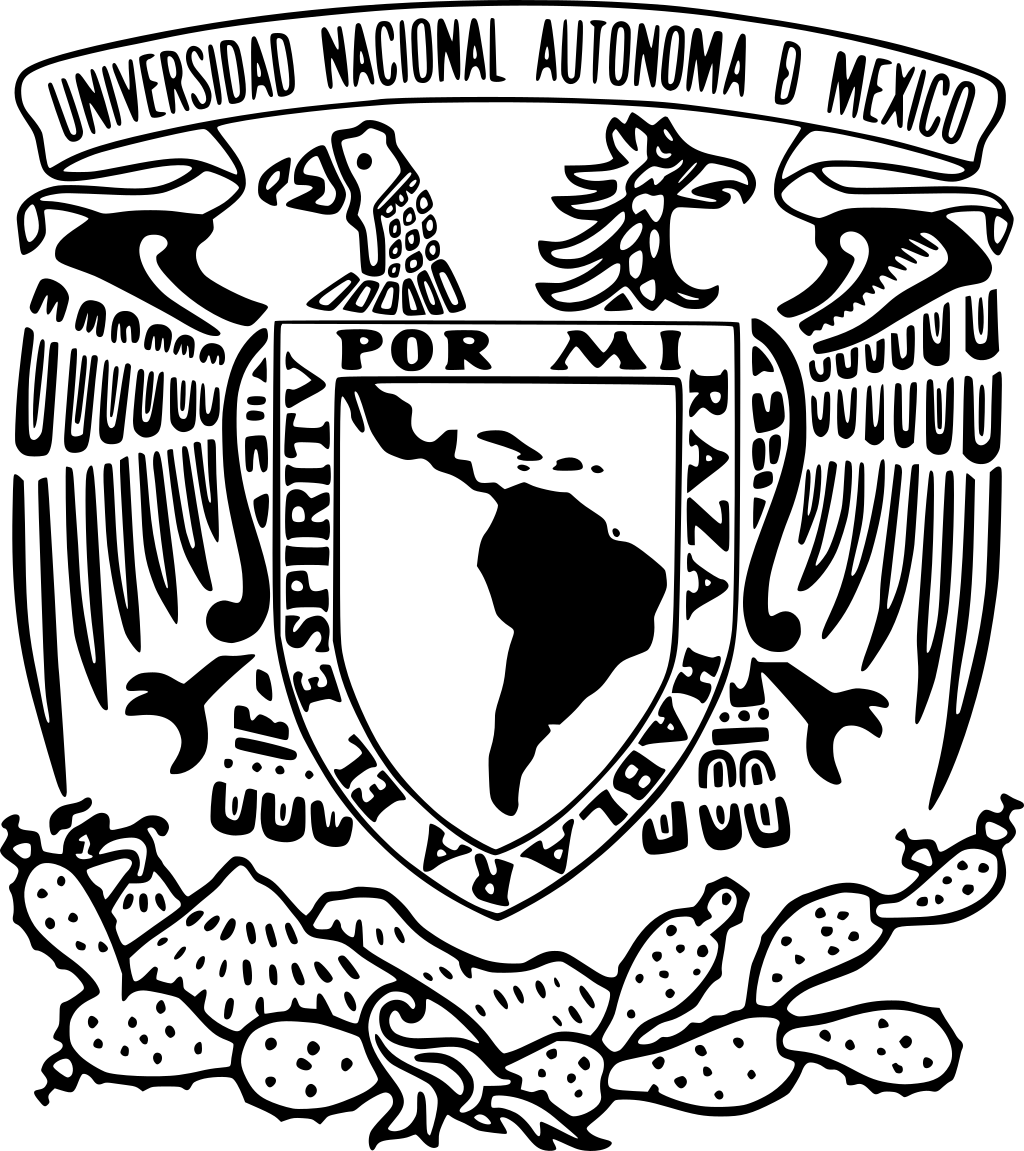
\includegraphics[width=2cm]{unam.png} \hspace{11.5cm}
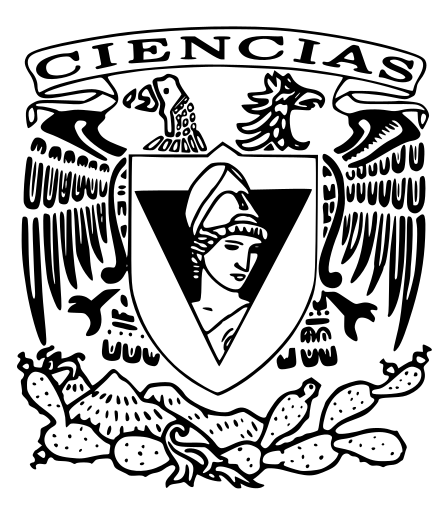
\includegraphics[width=2cm]{ciencias.png}\vspace{-2.2cm}
     {\scshape\Large Universidad Nacional Autónoma de México \par}
     {\scshape\Large Facultad de Ciencias, Ciudad Universitaria \par}
     {\Large Fundamentos de Bases de Datos 7063\par}
     \vspace{0.2cm}
     {\Large\bfseries Normalización de Base de Datos Transpórtate \par}
     \vspace{0.2cm}
     {\large\itshape Diego Alfredo Villalpando Velázquez \par \vspace{0.2cm}}
     {\large\itshape 13 de diciembre de 2019\par} \vspace{0.35cm}
     \noindent\hrulefill
}

%===========Objetivo===========%
\vspace{0.5cm}
       { \bfseries
         Objetivo:
         Se describe a continuación el proceso de normalización a tercera forma normal
         de la base de datos con estructura descrita anteriormente en el pdf anexo
         "disenio.pdf" sobre la empresa Transpórtate.
       }
       
       % Índice de contenido
       \noindent \tableofcontents

       %===========Introducción===========%
       
       \section{Introducción}
       {
         La empresa Transportate es una empresa de transporte particular con 150 automóviles
         propios para transporte de usuarios ajenos a la empresa y de forma individual. La
         empresa desea crear una base de datos que permita realizar estadísticas
         de los viajes e implementar un nuevo sistema de recompensas para sus clientes
         frecuentes. Se enumeran las reglas de negocio a continuación:
       }
       
       %===========Diseño E/R===========%
       \section{Nuevo Modelo Normalizado en 3NF}

       \subsection{Diagrama}

       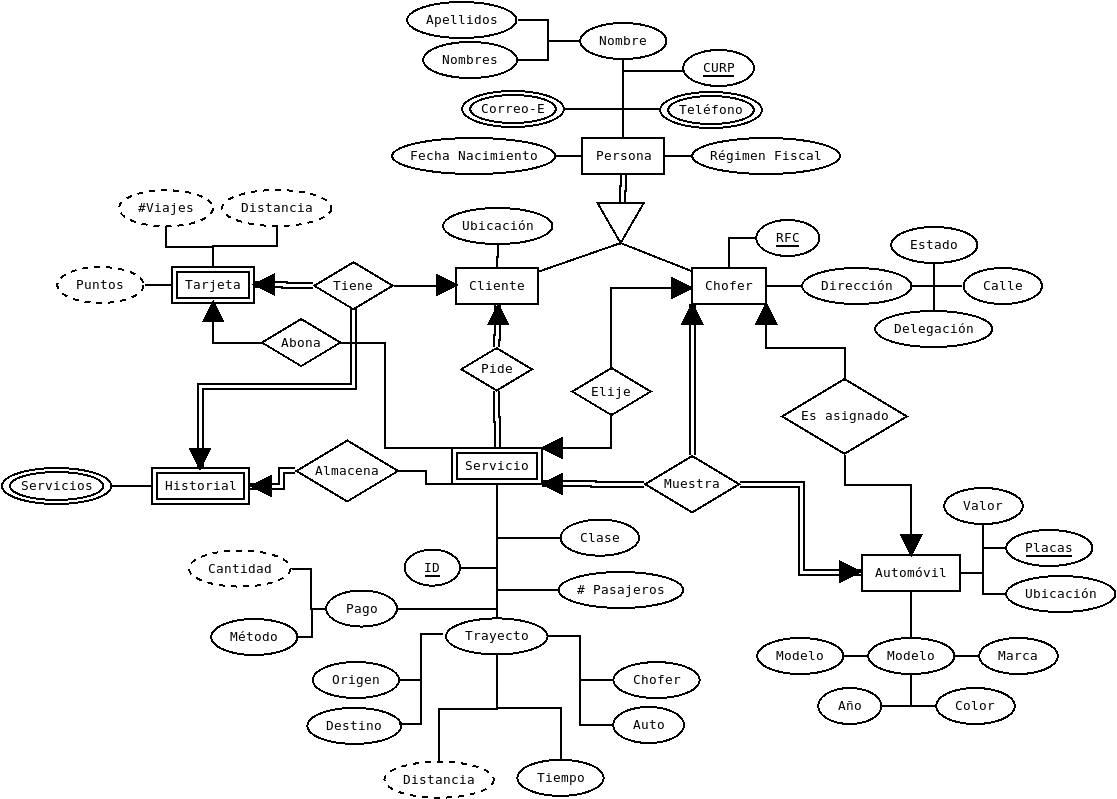
\includegraphics[width=15cm]{ER.png}\\
       \centerline{Diagrama 1: Modelo Relacional normalizado del caso.}\\

       \subsection{Justificación}

       \subsection{Procedimiento}
       \begin{enumerate}

       \end{enumerate}

       Dependencias Funcionales:
       \begin{itemize}

       \end{itemize}

       Llaves Primarias:
       \begin{itemize}

       \end{itemize}

       Llaves Secundarias:
       \begin{itemize}

       \end{itemize}

       Llaves Candidatas:
       \begin{itemize}

       \end{itemize}

       %===========Diseño Relacional===========%
       \section{Dominio y Restricciones de Tablas Normalizadas}

       \subsection{Clientes}
       \begin{tabular}{|l|l l c c c|} \hline
         Nombre              & Tipo        & Constraint     & PRIMARIA   & AJENA & NO NULO    \\ \hline
         CURP                & char(18)    & -              & \checkmark & -     & \checkmark \\ 
         Nombres             & text        & -              & -          & -     & \checkmark \\ 
         Apellidos           & text        & -              & -          & -     & \checkmark \\ 
         Fecha de nacimiento & date        & -              & -          & -     & \checkmark \\ 
         Régimen Fiscal      & char(1)     & CHECK(F||M||E) & -          & -     & -          \\ 
         Ubicación           & varchar(12) & -              & -          & -     & -          \\ \hline
       \end{tabular}\\ \vspace{1cm}

       \subsection{Choferes}
       \begin{tabular}{|l|l l c c c|} \hline
         Nombre              & Tipo        & Constraint     & PRIMARIA   & AJENA & NO NULO    \\ \hline
         CURP                & char(18)    & -              & \checkmark & -     & \checkmark \\ 
         RFC                 & char(22)    & -              & \checkmark & -     & \checkmark \\ 
         Nombres             & text        & -              & -          & -     & \checkmark \\ 
         Apellidos           & text        & -              & -          & -     & \checkmark \\ 
         Fecha de nacimiento & date        & -              & -          & -     & \checkmark \\ 
         Régimen Fiscal      & char(1)     & CHECK(F||E)    & -          & -     & \checkmark \\ 
         Calle               & text        & -              & -          & -     & \checkmark \\ 
         Delegación          & text        & -              & -          & -     & \checkmark \\ 
         Estado              & text        & -              & -          & -     & \checkmark \\ \hline
       \end{tabular}\\\vspace{1cm}

       \subsection{Automóviles}
       \begin{tabular}{|l|l l c c c|} \hline
         Nombre              & Tipo        & Constraint     & PRIMARIA   & AJENA      & NO NULO    \\ \hline
         Placas              & varchar(8)  & -              & \checkmark & -          & \checkmark \\ 
         RFC                 & char(22)    & -              & -          & \checkmark & \checkmark \\ 
         Marca               & text        & -              & -          & -          & \checkmark \\ 
         Modelo              & text        & -              & -          & -          & \checkmark \\ 
         Año                 & char(4)     & -              & -          & -          & \checkmark \\ 
         Color               & text        & -              & -          & -          & \checkmark \\ 
         Ubicación           & varchar(12) & -              & -          & -          & -          \\ 
         Valor               & money       & -              & -          & -          & \checkmark \\ \hline
       \end{tabular}\\\vspace{1cm}

       \subsection{Servicios}
       \begin{tabular}{|l|l l c c c|} \hline
         Nombre              & Tipo        & Constraint     & PRIMARIA   & AJENA      & NO NULO    \\ \hline
         ID\_Servicio        & big serial  & -              & \checkmark & -          & \checkmark \\ 
         CURP                & char(18)    & -              & -          & \checkmark & \checkmark \\ 
         RFC                 & char(22)    & -              & -          & \checkmark & \checkmark \\ 
         Placas              & varchar(8)  & -              & -          & \checkmark & \checkmark \\ 
         #Pasajeros          & smallint    & CHECK(8>x>0)   & -          & -          & \checkmark \\ 
         Origen              & varchar(12) & -              & -          & -          & \checkmark \\ 
         Destino             & varchar(12) & -              & -          & -          & \checkmark \\ 
         Tiempo              & time        & -              & -          & -          &            \\ 
         Distancia           & real        & CHECK(x>0)     & -          & -          & \checkmark \\ 
         Clase               & smallint    & CHECK(5>x>0)   & -          & -          & \checkmark \\ 
         Cantidad            & money       & -              & -          & -          & \checkmark \\ 
         Metodo              & bool        & -              & -          & -          & \checkmark \\ 
         Puntos\_Generados   & numeric     & CHECK(x>0)     & -          & -          & \checkmark \\ \hline
       \end{tabular}\\\vspace{1cm}

       \subsection{Correos-E}
       \begin{tabular}{|l|l l c c c|} \hline
         Nombre              & Tipo        & Constraint     & PRIMARIA   & ÚNICA      & NO NULO    \\ \hline
         CURP                & char(18)    & -              & \checkmark & \checkmark & \checkmark \\ 
         Direccion-E         & text        & -              & -          & \checkmark & \checkmark \\ \hline
       \end{tabular}\\\vspace{1cm}

       \subsection{Teléfonos}
       \begin{tabular}{|l|l l c c c|} \hline
         Nombre              & Tipo        & Constraint     & PRIMARIA   & ÚNICA      & NO NULO    \\ \hline
         CURP                & char(18)    & -              & \checkmark & \checkmark & \checkmark \\ 
         Telefono            & text        & -              & -          &            & \checkmark \\ \hline
       \end{tabular}\\\vspace{1cm}

       \subsection{Historial}
       \begin{tabular}{|l|l l c c c|} \hline
         Nombre              & Tipo        & Constraint     & PRIMARIA   & ÚNICA      & NO NULO    \\ \hline
         CURP                & char(18)    & -              & \checkmark & \checkmark & \checkmark \\ 
         ID\_Servicio        & bigserial   & -              & -          & \checkmark & \checkmark \\ \hline
       \end{tabular}\\\vspace{1cm}
       
       \subsection{Tarjeta}
       \begin{tabular}{|l|l l c c c|} \hline
         Nombre              & Tipo        & Constraint     & PRIMARIA   & ÚNICA      & NO NULO    \\ \hline
         CURP                & char(18)    & -              & \checkmark & \checkmark & \checkmark \\ 
         Distancia           & real        & CHECK(x>0)     & -          &            & \checkmark \\ 
         Puntos              & numeric     & CHECK(x>0)     & -          &            & \checkmark \\ 
         #Viajes             & numeric     & CHECK(x>0)     & -          &            & \checkmark \\ \hline
       \end{tabular}\\\vspace{1cm}
       
       
        %===========Bibliografía===========%
       \newpage
           {\noindent \section*{Bibliografía}}
           
           {\noindent
             [1] The PostgreSQL Global Development Group (2019). {\bfseries Chapter 8. Data Types},
             {\itshape PostgreSQL}.
             En linea. Accesado el 10 de diciembre de 2019.
             (\url{https://www.postgresql.org/docs/current/datatype.html}).
             \par \vspace{0.3cm}
           }\\
           
\end{document}
